\section{Thesis outline}

All organisms in nature tirelessly perform work, struggling against an ever increasing
entropy. \todo{betere openingszin} This work is collectively performed by countless
molecular machines, all contributing their specific task. On the length-scales of these
machines, often times not larger then a few nanometres, the dominant forces result from
random thermal fluctuations.

These thermal fluctuations result in the stochastic motion of these
molecular structures.


No work can be extracted from
freely tumbling, randomly oriented molecules.  This
fundemental limit has been overcome by interfacing synthetic molecular machines
with surfaces.

Most commonly known is the bacterial flagella motor, providing an efficient way for
bacteria to roll and tumble around


work by the flow of cations through the stator
which transiently changes the electorstatic interaction between the stator and the rotor
to generate unidirectional torque --> NO ATP!

synthetic is difficult. dissipating heat, soft large structures.  polymers, DNA.

DNA piston can be characterised as a autonomous molecular machine, which turns
over chemical fuel to perform work continuously. bayoumi et al.

aim of the molecular machine is to perform selective transport of dna through the
membrane. This has been done before following an external bias, but special is that the
machine opperates also opposing a external bias. The physics that makes this special
property possible is entropy and will be discussed futher in detail in later chapters of
this thesis.

thesis outline, first chapter is a short introduction to important concepts. chapter two
is a discussion of the dna nanopiston, largely based on the paper recently published by
bayoumi et al. Next adaptation of the model is discussed in chapter 3. The results of
these simulations are discussed in the last chapter.

\begin{figure}
\begin{center}
  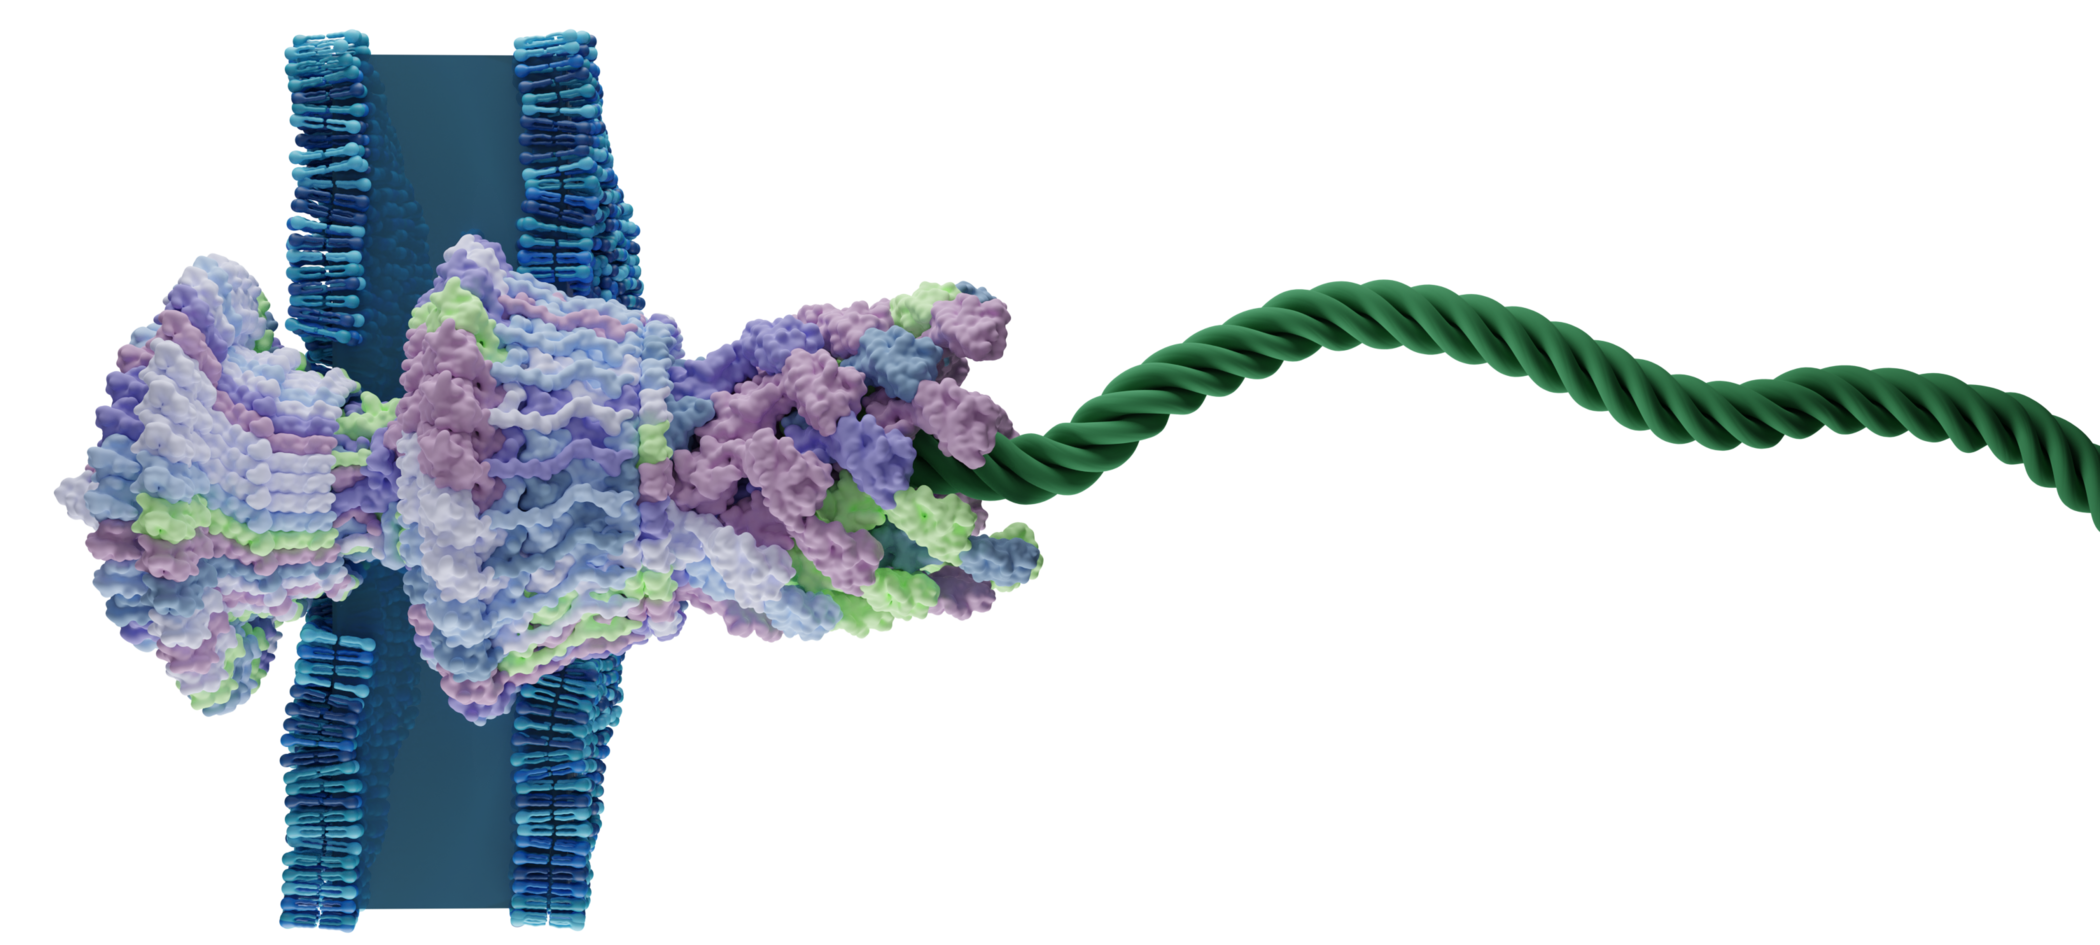
\includegraphics[width=0.80\textwidth]{Figures/flagella.png}
  \caption{write caption}
\end{center}
\end{figure}
